\section{问题三的模型建立与求解}

\subsection{模型建立}

问题三固定题目给定的AI与非AI IT负荷，不调整任务区域和开工时刻，仅优化新能源分配、储能充放电及购售电，以识别储能的能源侧作用。

设区域$r$在时段$t$的设施负荷为$F_{rt}$，
可用新能源功率为$P^{RE}_{rt}$，
电网购电功率为$B_{rt}$；
新能源直接供能、新能源充电、电网充电、储能放电、
新能源外送和弃用功率分别记为
$V_{rt}$、$C^{RE}_{rt}$、$C^G_{rt}$、
$D_{rt}$、$X_{rt}$和$R_{rt}$。
设施负荷与逐时能源平衡满足
\begin{equation}
	\begin{aligned}
		F_{rt}
		&=
		PUE_r
		\left(
		P^{AI}_{rt}+P^{NonAI}_{rt}
		\right),\\
		P^{RE}_{rt}
		&=
		V_{rt}+C^{RE}_{rt}+X_{rt}+R_{rt},\\
		B_{rt}+V_{rt}+D_{rt}
		&=
		F_{rt}+C^G_{rt}.
	\end{aligned}
	\label{eq:q3_energy_balance}
\end{equation}

其中$F_{rt}$已知，且$0\leq V_{rt}\leq F_{rt}$、$0\leq C^G_{rt}\leq B_{rt}$。

设$S_{rt}$为时段$t$开始时的储能电量。数据中心储能调度通常依据SOC递推和功率边界实现跨时调节\cite{ref10}；本文进一步加入充放电互斥、购售电边界和终端SOC约束，进行全时域求解。
时间步长为1 h，充、放电效率分别为$\eta_r^c$和$\eta_r^d$，
则SOC递推为
\begin{equation}
	S_{r,t+1}
	=
	S_{rt}
	+
	\eta_r^c
	\left(
	C^{RE}_{rt}+C^G_{rt}
	\right)
	-
	\frac{D_{rt}}{\eta_r^d}.
	\label{eq:q3_soc}
\end{equation}

储能满足容量、功率及$S_{r,2406}\geq S_{r0}$；引入$y_{rt}\in\{0,1\}$排除同时充放电：
$C^{RE}_{rt}+C^G_{rt}\leq y_{rt}P_r^{ch,\max}$、
$D_{rt}\leq(1-y_{rt})P_r^{dis,\max}$。
购电满足$0\leq B_{rt}\leq P_r^{Grid,\max}$；新能源外送满足$0\leq X_{rt}\leq\bar X_r$及$X_{rt}\leq P_r^{Grid,\mathrm{out},\max}$。

沿用问题二的成本和碳排放口径，并增加峰值净购电与净购电波动指标。
定义区域净购电功率$N_{rt}=B_{rt}-X_{rt}$，
则
\begin{equation}
	\begin{aligned}
		C&=
		\sum_r\sum_t
		\left(
		\pi_{rt}B_{rt}-\sigma_{rt}X_{rt}
		\right),\\
		E&=
		\sum_r\sum_t
		\kappa_{rt}B_{rt},\\
		P&=
		\sum_rP_r^{\max},
		\qquad
		P_r^{\max}\geq N_{rt},\quad
		P_r^{\max}\geq0,\\
		W&=
		\frac{1}{6(T-1)}
		\sum_r\sum_tW_{rt}.
	\end{aligned}
	\label{eq:q3_objectives}
\end{equation}

其中$t=0,\ldots,2405$，$T=2406$；$W_{rt}\geq\pm(N_{r,t+1}-N_{rt})$，故$W$为相邻小时净购电的平均绝对变化量，$P_r^{\max}\geq0$避免将净外送解释为负峰值。

四项指标量纲不同且无给定权重，先求单目标理想值$f_m^{best}$，再将各单目标方案$x^{(j)}$代入全部指标，取$f_m^{ref}=\max_j f_m(x^{(j)})$。
对于存在有效权衡关系的指标，定义
\begin{equation}
	\bar f_m
	=
	\frac{f_m-f_m^{best}}
	{f_m^{ref}-f_m^{best}}.
	\label{eq:q3_normalization}
\end{equation}

若$f_m^{ref}=f_m^{best}$，该指标仅用于评价；其余指标采用三级择优：
\begin{equation}
	\begin{aligned}
		&\text{第一级：}\quad
		\min z,
		\qquad
		\bar f_m\leq z;\\
		&\text{第二级：}\quad
		\min \Phi=\sum_m\bar f_m;\\
		&\text{第三级：}\quad
		\min G=
		\sum_r\sum_t
		\left(
		C^{RE}_{rt}+C^G_{rt}+D_{rt}
		\right).
	\end{aligned}
	\label{eq:q3_multilevel}
\end{equation}

前两级控制最大偏离和总偏离，第三级在近等价方案中减少无意义循环。除充放电互斥外均为线性约束，故直接求解第0--2405小时混合整数线性规划，并在2406检查终端SOC。


\subsection{求解结果与模型检验}

六区域统一求解结果见图\ref{fig:q3_storage}：RegionA--RegionC基本不充放电，调节集中于RegionD--RegionF。
RegionD的SOC约为$90.0\sim712.4$ MWh，
RegionE和RegionF分别约为
$82.0\sim820.0$ MWh和$85.0\sim850.0$ MWh，
SOC变化与式(\ref{eq:q3_soc})中的充放电状态保持一致。

\begin{figure}[H]
	\centering
	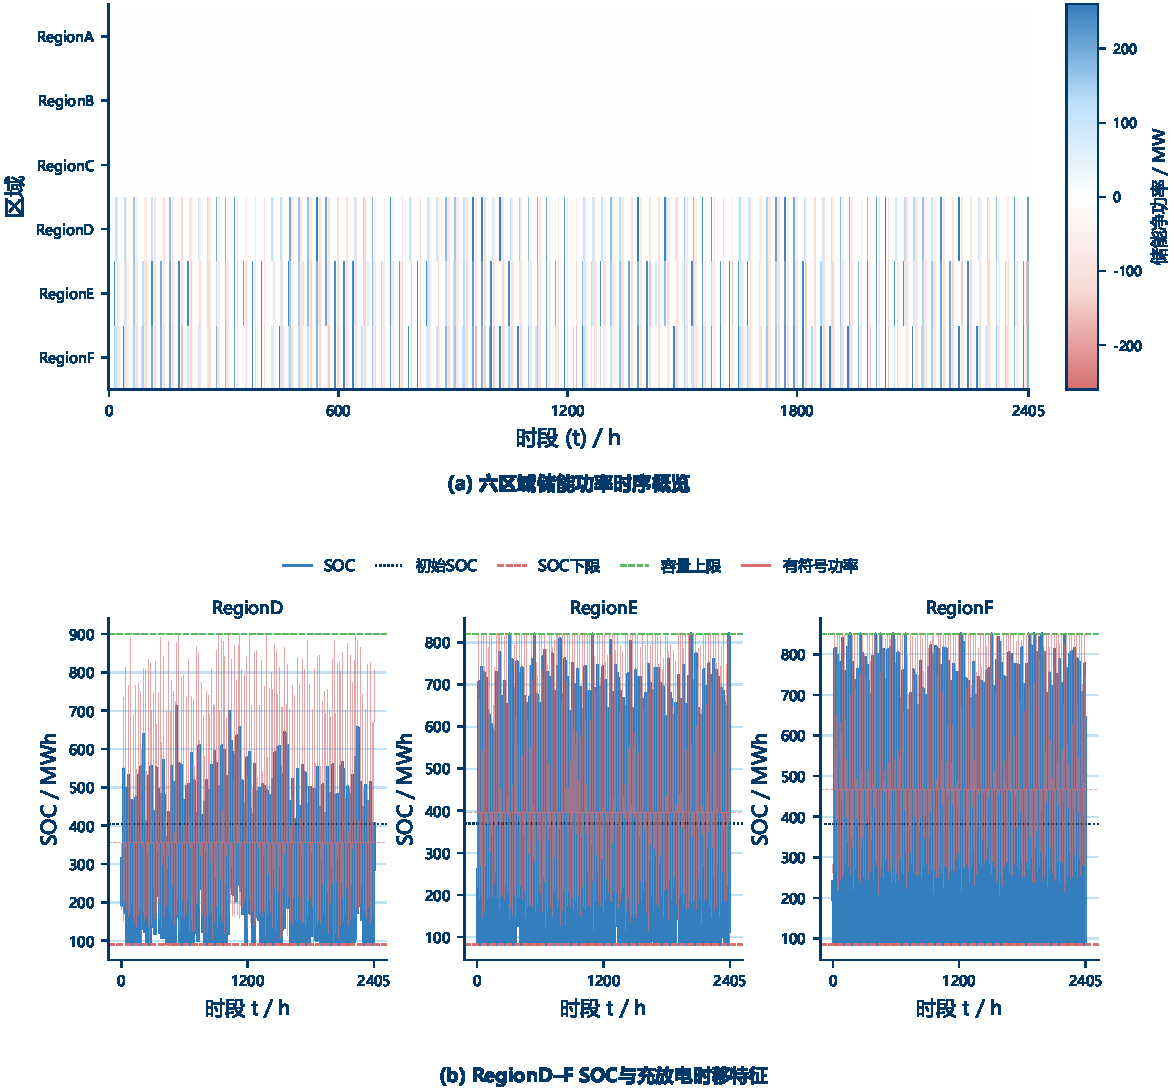
\includegraphics[width=0.92\textwidth]
	{figures/q3_group1_storage_mechanism.pdf}
	\caption{六区域储能功率时序与活跃区域SOC演化特征}
	\label{fig:q3_storage}
\end{figure}

储能由此集中配置于调节需求较强的区域，而非各区域均匀调用。

题目附件状态仅作实际运行对照，不作为满足本文终端SOC条件的同可行域优化基准；无储能方案用于同模型口径消融。
优化后运行成本为
$C=-4.5906\times10^{8}$，
碳排放$E=0$，
六区域峰值净购电之和$P=0$，
平均净购电波动$W=0.0113$ MW。
四项指标均优于附件对照；负成本表示外送收益超过购电支出。

碳排放和峰值净购电均为0，并不表示数据中心没有电力负荷。按照题目给定口径，碳排放仅由电网购电量计算，峰值指标取净购电功率的正部；在当前确定性数据和允许新能源外送的边界下，优化方案利用新能源和储能满足负荷，并将富余新能源外送，因而购电碳排放和正向净购电峰值均降至0。该结论依赖当前新能源、电价、储能和购售电边界，不代表其他参数情景下仍能保持为0。

\begin{figure}[H]
	\centering
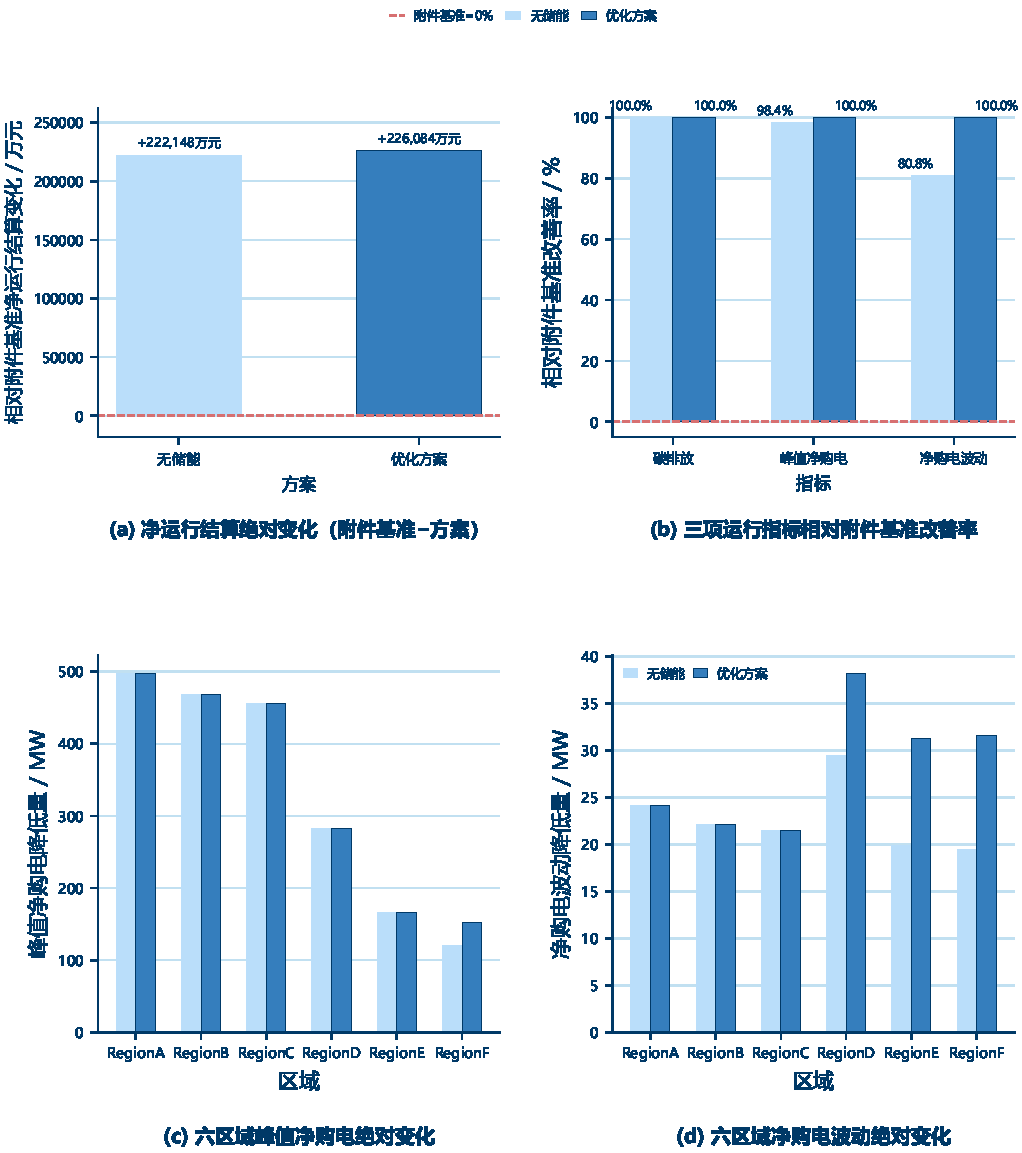
\includegraphics[width=0.86\textwidth]
{figures/q3_group2_optimization_effect.pdf}
\caption{储能协同优化的净运行结算绝对变化、三项指标改善率与区域差异}
	\label{fig:q3_effect}
\end{figure}

图\ref{fig:q3_effect}以万元表示净运行结算绝对变化，以相对改善率表示其余指标，避免成本跨零时的比例歧义。六区域峰值均下降，RegionD--RegionF波动改善更大，与储能活跃区域一致。

令$C^{RE}_{rt}=C^G_{rt}=D_{rt}=0$构造无储能反事实方案。
其运行成本为$-4.1969\times10^{8}$，
碳排放为$8.8506$，
峰值净购电为$31.5979$ MW，
平均净购电波动为$5.3981$ MW。
与其相比，优化方案的净运行成本降低3936.19万元，碳排放、峰值和波动也下降。

独立复核表明，优化方案与无储能方案均满足能源平衡、SOC、容量、互斥、购售电及终端约束。
附件运行对照的新能源平衡和负荷平衡最大残差分别约为
$2.0\times10^{-4}$ MW和$1.504\times10^{-4}$ MW，
处于原始数据精度量级；
但SOC递推最大偏差约为$0.9999$ MWh，
终端SOC缺口约为$193.3$ MWh。
故附件状态可作题设运行对照，但不属于本文约束下的可行优化解。

\begin{figure}[H]
	\centering
	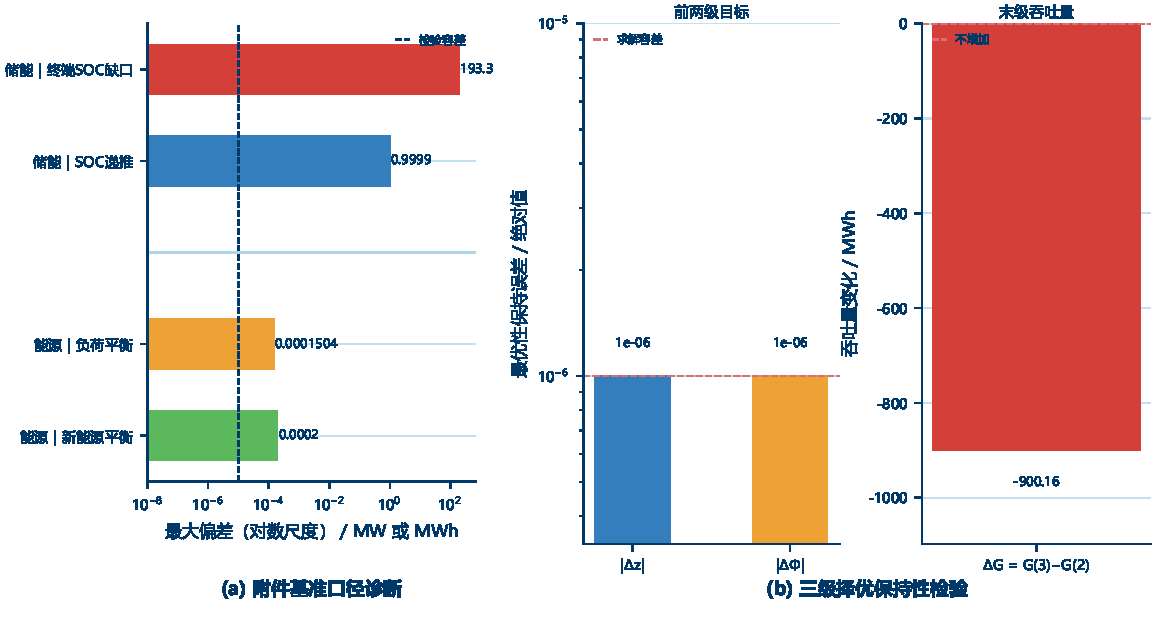
\includegraphics[width=0.91\textwidth]
	{figures/q3_group3_validation_credibility.pdf}
	\caption{附件运行对照口径诊断与多目标三级择优检验}
	\label{fig:q3_validation}
\end{figure}

图\ref{fig:q3_validation}中，第三级使$z$和$\Phi$相对前一级的变化均约$1.0\times10^{-6}$，储能吞吐量减少900.16 MWh，即在保持前两级结果时减少无效循环。

问题三在固定负荷下量化储能的跨时调节作用，并为问题四提供能源侧基准。



\section{问题四的模型建立与求解}

\subsection{模型建立}

问题四联合优化任务区域、开工时刻、新能源、储能及购售电。以问题二可行任务方案为初始方案，沿用问题三能源机理；任务迁移和错峰经PUE映射影响新能源消纳、SOC和电网交换，因而建立算--储--电联合模型。

负荷空间迁移与时间调整可同储能及电力决策联动\cite{ref9}。本文保留任务时限、网络时延、资源容量和能源边界，并设置终端SOC与滚动可恢复约束。

任务侧沿用问题一可行域。由$x_{irs}$和式(\ref{eq:q1_overlap})得到AI IT负荷
$P_{rt}^{AI}=\sum_i\sum_{s\in S_i}p_i\rho_{ist}x_{irs}$，
设施侧负荷为
$F_{rt}=PUE_r(P_{rt}^{AI}+P_{rt}^{NonAI})$。
任务唯一执行，实时任务立即启动，弹性任务满足时窗、时延、GPU、功率及2406边界。

能源侧沿用式(\ref{eq:q3_energy_balance})和式(\ref{eq:q3_soc})及其容量、互斥、购售电与外送约束，并要求$S_{r,2406}\geq S_{r0}$。

为防止滚动求解在前期过度放电，还在每个决策窗口末端加入SOC可恢复条件：
\begin{equation}
	S_{r,\tau+H}
	\geq
	\max\left\{
	S_r^{\min},
	S_{r0}-
	\eta_r^cP_r^{ch,\max}(2406-\tau-H)
	\right\}.
	\label{eq:q4_soc_recovery}
\end{equation}

式(\ref{eq:q4_soc_recovery})保证剩余时域仍有恢复初始SOC的理论能力，并在终点衔接终端约束。

六项评价指标为净运行结算$C$、碳排放$E$、网络时延$L$、等待损失$J$、新能源未利用率$Q$和峰值净购电$P$。前三项口径沿用问题二、三；设弹性任务合法开工边界为$\underline{s}_i,\overline{s}_i$，时延敏感权重为$\omega_i$，则
\begin{equation}
	\begin{aligned}
		J&=
		\frac{
			\displaystyle\sum_{i\in I^{\mathrm{flex}}_+}
			\omega_i
			\frac{s_i-\underline{s}_i}
			{\overline{s}_i-\underline{s}_i}}
		{\displaystyle\sum_{i\in I^{\mathrm{flex}}_+}\omega_i},
		\qquad QoS=1-J,\\
		Q&=
		\frac{\displaystyle\sum_r\sum_tR_{rt}}
		{\displaystyle\sum_r\sum_tP^{RE}_{rt}},
		\qquad U=1-Q,\\
		P&=\sum_rP_r^{\max},
		\qquad
		P_r^{\max}\geq B_{rt}-X_{rt},
		\quad P_r^{\max}\geq0.
	\end{aligned}
	\label{eq:q4_metrics}
\end{equation}

滚动求解前固定全局中心$a_m$和尺度$R_m$，各窗口和情景不再改变；非退化主动指标集合为$\mathcal M_{\mathrm{act}}=\{L,J,Q\}$。
第$\tau$个窗口的标准化偏离和增广极小极大准则为
\begin{equation}
	\begin{aligned}
		d_{m,\tau}
		&=
		\max\left\{
		0,\,
		\frac{\hat f_{m,\tau}-a_m}{R_m}
		\right\},
		\qquad m\in\mathcal M_{\mathrm{act}},\\
		\min\quad Z_\tau
		&=
		z_\tau+\eta\sum_{m\in\mathcal M_{\mathrm{act}}} d_{m,\tau},
		\qquad
		d_{m,\tau}\leq z_\tau\quad(m\in\mathcal M_{\mathrm{act}}),
		\qquad
		\eta=10^{-3}.
	\end{aligned}
	\label{eq:q4_minmax}
\end{equation}

式(\ref{eq:q4_minmax})仅对$\mathcal M_{\mathrm{act}}$计算；$C,E,P$独立复算，用于评价和情景比较。六项指标构成统一评价体系，但并非同等强度的主动优化目标。

全时域联合整数变量规模过大，故采用问题二初始方案驱动的滚动数学启发式：$H=24$ h、$K=48$ h、内部推进4 h，前瞻区只提供未来信息。流程见表\ref{tab:q4_algorithm}。

% ==================== Q4：滚动求解流程 ====================
\begin{table}[H]
	\centering
	\caption{问题四滚动算--储--电联合求解流程}
	\label{tab:q4_algorithm}
	
	\fontsize{10.5pt}{12pt}\selectfont
	\renewcommand{\arraystretch}{0.88}
	
	\begin{tabular}{
			>{\centering\arraybackslash}p{0.08\textwidth}
			>{\raggedright\arraybackslash}p{0.86\textwidth}}
		\toprule
		\textbf{步骤} & \multicolumn{1}{c}{\textbf{主要操作}}\\
		\midrule
		
		1 & 读取问题二任务种子及当前SOC、历史峰值和剩余任务状态。\\
		
		2 & 在$H=24$ h决策区和$K=48$ h前瞻区内重新求解储能与购售电响应。\\
		
	3 & 利用边际线性规划评价弹性任务迁移、错峰对联合目标的潜在影响。\\
		
	4 & 对产生资源冲突的局部调整调用小规模混合整数线性规划模型进行可行性修复。\\
		
	5 & 选取关键任务组成大邻域，同时开放任务与能源变量进行联合大邻域搜索精修。\\
		
		6 & 提交当前$H$小时可行结果，并更新SOC、历史峰值、累计碳排放及剩余任务。\\
		
		\bottomrule
	\end{tabular}
\end{table}


联合大邻域同时开放任务区域、开工时刻和能源变量，仅接受满足全部硬约束且使式(\ref{eq:q4_minmax})目标值改善的方案。所得结果为严格满足硬约束且计算效率较高的可行方案，不宣称获得全局最优解。

顺序基准固定问题二任务方案，再按问题三能源模型优化储能和购售电；两方案采用相同六项指标。

保持任务、网络、容量和储能参数不变，分别改变碳约束、电价机制和新能源波动。设基准碳排放为$E^0$、低碳参考为$E^{LC}$，新能源平滑参数为$\gamma$，三类情景定义为
\begin{equation}
	\begin{aligned}
		E
		&\leq
		E^0-\lambda(E^0-E^{LC}),
		\qquad 0\leq\lambda\leq1,\\
		\pi_{rt}^{fix}
		&=\bar{\pi}_r,
		\qquad
		\sigma_{rt}^{fix}=\bar{\sigma}_r,\\
		P_{rt}^{RE}(\gamma)
		&=
		(1-\gamma)P_{rt}^{RE}
		+\gamma\bar P_{rd}^{RE,+},
		\qquad
		t\in\mathcal H_{rd}^{+}.
	\end{aligned}
	\label{eq:q4_scenarios}
\end{equation}

新能源平滑仅作用于原非零时段并保持每日总量，所有情景沿用固定定标尺度。

最终由任务表和完整SOC轨迹重构第0--2405小时剖面，统一复算六项指标及全部硬约束。

\subsection{求解结果与模型检验}

采用$H=24$ h、$K=48$ h对50000个任务完成101个滚动窗口，仅提交满足全部硬约束的决策区结果，并在全时域统一复算。

旧顺序能源解因报告型指标退化而形成了物理意义较弱的比较基准。为消除该影响，本文固定问题二顺序任务方案和既有联合任务方案，均按相同的能源响应规则重新优化储能与购售电。该步骤仅统一复算两套任务方案的能源轨迹，不等同于重新执行完整联合搜索。结果见表\ref{tab:q4_result}。

% ==================== Q4：联合方案结果 ====================
\begin{table}[H]
	\centering
	\caption{统一能源口径下联合任务方案与顺序任务方案对比}
	\label{tab:q4_result}
	
	\fontsize{10.5pt}{12pt}\selectfont
	\renewcommand{\arraystretch}{0.90}
	
	\begin{tabular}{lrr}
		\toprule
		\multicolumn{1}{c}{\textbf{评价指标}}
		& \multicolumn{1}{c}{\textbf{顺序任务方案}}
	& \multicolumn{1}{c}{\textbf{联合任务方案}}\\
		\midrule
		
		净运行结算/元
		& $-4.532307\times10^8$
		& $-4.538873\times10^8$\\
		
		碳排放/tCO$_2$
		& 30.1233
		& 71.2005\\
		
		平均网络时延/ms
		& 12.9468
		& 9.9618\\
		
		QoS损失
		& 0.083659
		& 0.079281\\
		
		新能源未利用率
		& 29.8615\%
		& 29.8357\%\\
		
		峰值净购电/MW
		& 66.5709
		& 97.1828\\
		
		\bottomrule
	\end{tabular}
\end{table}


表\ref{tab:q4_result}中，联合任务方案的净运行结算降低$6.5665\times10^5$元，时延下降2.9851 ms，QoS损失下降0.004378，新能源未利用率降低0.0258个百分点；碳排放增加41.0772 tCO$_2$，峰值净购电增加30.6119 MW。负结算表示外送收益超过购电支出。结果表明，联合任务调整主要改善服务质量并小幅降低净结算和弃新能源，但未使六项评价指标同时改善。

因此，两类方案不存在脱离决策偏好的统一优劣关系。若调度者优先改善网络时延、等待损失和新能源消纳，并能接受相应的碳排放与峰值净购电增量，则可采用联合任务方案；若碳排放或峰值净购电属于严格控制指标，则应采用相应约束情景下的方案。本文据此将结果解释为不同运行偏好下的可行策略集合，而不指定脱离应用条件的唯一最优方案。

\begin{figure}[H]
	\centering
	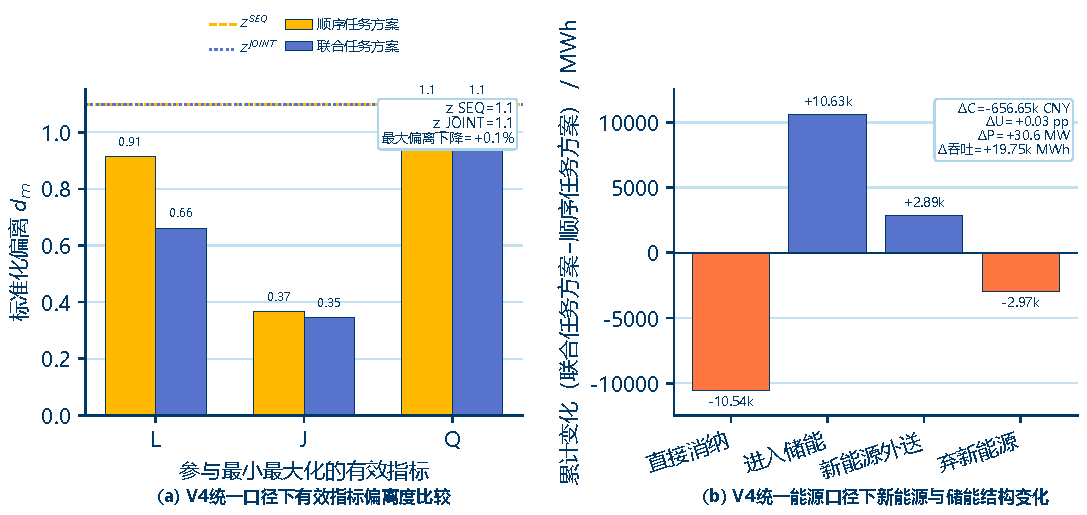
\includegraphics[width=0.88\textwidth]
	{figures/q4_group1_joint_optimization_results.pdf}
	\caption{统一能源口径下两类任务方案的有效指标与新能源--储能结构对比}
	\label{fig:q4_joint_result}
\end{figure}

图\ref{fig:q4_joint_result}中，联合任务方案相较顺序任务方案的新能源直接消纳减少$10.54\times10^3$ MWh，储能充入和外送分别增加$10.63\times10^3$、$2.89\times10^3$ MWh，弃新能源减少$2.97\times10^3$ MWh，储能吞吐量增加$19.75\times10^3$ MWh。图中$L,J,Q$为既有联合搜索实际采用的非退化主动指标；$C,E,P$按统一能源口径独立复算，用于报告任务方案的能源侧代价，不将其追溯表述为联合搜索目标。

按式(\ref{eq:q4_scenarios})构造碳约束、平价电价和新能源平滑情景，相对联合基准的变化见图\ref{fig:q4_scenario}。该图沿用已完成情景组及其同版本联合基准，仅比较组内相对响应；表\ref{tab:q4_result}与图\ref{fig:q4_joint_result}的定点能源复算专用于纠正顺序--联合方案比较，两类结果不交叉拼接绝对量。

\begin{figure}[H]
	\centering
	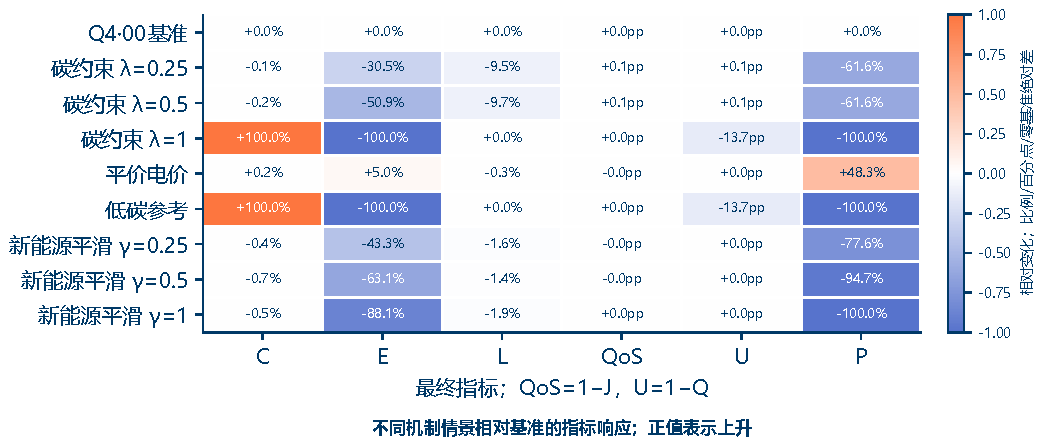
\includegraphics[width=0.86\textwidth]
	{figures/q4_group2_scenario_response.pdf}
	\caption{不同机制情景相对问题四基准的指标响应}
	\label{fig:q4_scenario}
\end{figure}

图\ref{fig:q4_scenario}中，$\lambda$由0.25增至0.50时，碳排放由297.36降至209.97 tCO$_2$，峰值约95.54 MW，时延由9.0144变为8.9945 ms。
当$\lambda=1$时，碳排放和峰值净购电接近0，
但新能源未利用率升至43.5710\%，
即继续压缩购电会牺牲新能源利用，并非各指标同步改善。

平价电价下碳排放449.37 tCO$_2$、峰值升至368.71 MW。新能源平滑情景中，
当$\gamma=0.25,0.50,1.00$时，
碳排放分别约为242.89、158.01和50.85 tCO$_2$，
峰值净购电分别约为55.73、13.18和0 MW，
时延均为9.77--9.81 ms，表明平滑主要改变能源侧状态。

采用全时域独立复算和代表窗口完整混合整数线性规划检验。顺序任务方案与联合任务方案各67项任务、容量、时延、能源、SOC及购售电复核均通过，最大硬约束违反量为
$2.3842\times10^{-7}$，低于$10^{-6}$的检验容差；
六项指标独立复算后与汇总结果的最大差异亦不超过该量级。

\begin{figure}[H]
	\centering
	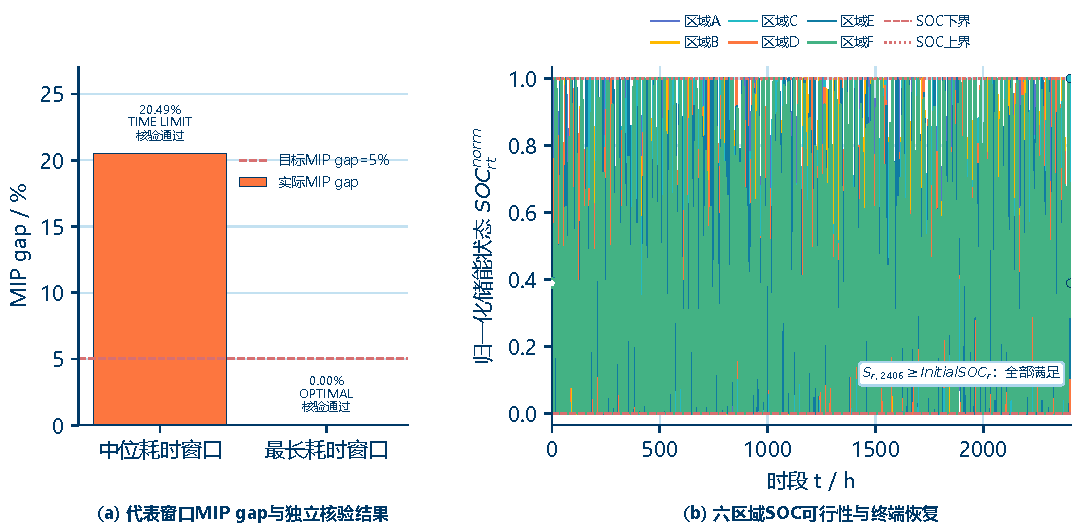
\includegraphics[width=0.88\textwidth]
	{figures/q4_group3_model_validation.pdf}
	\caption{问题四代表窗口完整混合整数线性规划与六区域储能状态的独立检验结果}
	\label{fig:q4_validation}
\end{figure}

图\ref{fig:q4_validation}(a)对1512和2232窗口作完整联合混合整数线性规划对照：前者在600 s内得到相对间隙20.49\%的可行参考解，后者达到最优，二者约束复核均通过。该检验只提供局部可行性与有限解质量参照，不能证明全时域近优或全局最优。

图\ref{fig:q4_validation}(b)给出联合任务方案按统一能源核算口径复算后的SOC轨迹。SOC始终位于上下界内，且$S_{r,2406}\geq S_{r0}$，未通过透支初始储能获取收益。

问题四的联合任务方案在当前数据下改善网络时延、等待损失和新能源未利用率，同时使碳排放与峰值净购电增加，说明联合决策产生的是指标权衡而非六项同步占优。两套任务方案均满足任务、算力、能源和储能硬约束；其结论限于严格满足硬约束且计算效率较高的可行方案，不宣称获得全局最优解，也不将能源定点复算等同于完整联合搜索。



